\section[Implementation, Integration and Test Plan]{\hyperlink{toc}{Implementation, Integration and Test Plan}}
	\label{sec:iitPlan}
	
	In this section we are going to provide a precise plan of how the implementation, integration and test plan should be realized in order to deal with all the characteristics and features of our system, now that we have a complete and clear description of all its aspects.\\
	
	First we provide a brief introduction of some entry conditions that must be met before starting with this plan, in particular with also some details of the tools we suggest to carry the process. Second, to accomplish some of the requirements of the system and to justify some other decision taken while defining the plan, we illustrate thanks to an \textbf{utility tree} the importance of the features we expect SafeStreets to provide. Finally, in the plan definition section (\ref{sec:planDefinition}) we give the precise description of how the \emph{Implementation, Integration and Test Plan} with a concise correspondence of the \textbf{use relation hierarchy} diagram (\autoref{fig:useRelationHierarchy}).
	
	\subsubsection[Strategy Overview]{\hyperlink{toc}{Strategy Overview}}
		\label{sec:strategyOverview}
		
		The system we have identified has its main complexity in the component that deals with the computation of all the requests coming from the users whenever a functionality is required. This is the reason why, while describing the component view section (\ref{sec:componentView}), we did not stop to identify only the components that compose the server one, but we deepened also inside each of them to understand how each of their functionality could be carried out. In this section we want to identify a plan to be followed while building the entire system, hence it is obvious that we will start from the \emph{Server Component}, in particular with the component that has to deal with the most critical feature inside of it. The plan will take in consideration only the first level of components the server is composed of, in fact, the more specific ones have been identified to provide an additional separation as it can be easier, for the team that is going to implement it, to chose how to proceed in their realization. This freedom inside the development of each component allows to obtain a better result having already identified the specific modules that will compose it; however, the implementation and testing of each component must always follow the plan that is later described.\\
		
		Thanks to what we have just identified we now list the main features we have considered for the \emph{Implementation, Integration and Test Plan}:
		
		\begin{itemize}
			\item \textbf{Bottom-Up and Top-Down:} we mainly focused on a bottom-up approach to define the plan because we decided to start from the basic components that compose the most critical one (the server) and then started to proceed upwards ending with the interactions of the entire system with the external ones. A top-down approach is also used in the cases where the realization of a component precedes the one that allows to manage its data. For example, the integration of the AccidentsManager component with the ACI is going to be done at the end of the plan as we can create mocked accidents to develop the main functionality that is the storing inside the database as they can be used for the safety calculus.
			
			\item \textbf{Core Functionality:} we consider the notification process the core functionality of our system, hence the most important to be first implemented, tested and integrated. Its realization will be held only after the \emph{DataManager Component} that allows us to manage the data of the system as soon as possible; the data needed to test the system will be mocked exploiting the top-down approach.
			
			\item \textbf{Decoupling of Components:} we have defined our plan with an interaction between the components that is mainly defined by the functionalities we want to realize. This means that the components needed to realize different functionalities can be considered first at the step of the realization of a functionality and left uncompleted until the others functionalities are taken into account.
			
			\item \textbf{Reliability of External Systems:} while considering the realization of the interaction with the external systems we do not take in consideration the testing of the methods provided by their interfaces as they should be already tested and verified by their providers. 
		\end{itemize}
	
	\subsubsection[Entry Criteria]{\hyperlink{toc}{Entry Criteria}}
		\label{sec:entryCriteria}
		
		The following conditions have to be met before entering the \emph{Implementation, Integration and Test Plan} as its guideline can be easily followed and meaningful results are obtained.\\
		
		A fundamental criterion on which the entire plan has to rely on is that the implementation goes in parallel with the testing. This consideration allows to retrieve the problems of the system as soon as possible nd to reduce the cost of their correction if found later; the percentage of testing for each module implemented has to be at lest 85\% in order to proceed with its integration.\\
		
		Another important issue related to the top-down approach often used in order to start developing the most critical components related to the most important functionalities of the system, is that we need to be able to generate feasible \textbf{stubs} that can be used to simulate the real data the system is going to manage. Hence some random generators may be also needed in order to consider all the possible cases in which the system can be stressed.\\
		
		Before starting with the identification of the plan we want to give some guidelines related to some very useful tools that can be used when the process of development and testing of the system really starts.
		
		\paragraph{Development Tools} We consider \emph{Java} as the main language the system has to be developed with. Thanks to its enormous popularity lots of documentations and libraries can be found to solve almost every of the problems we should encounter. In particular it fits also very well with the communication among different platforms and devices as in our case. In fact several editions have been released in order to deal with all the possible types of systems that can be developed.
		
		\paragraph{Testing Tools} Testing tools are fundamental in order to proceed with a correct and meaningful testing process while developing the system. Several tools are needed in order to consider all the testing issues, between all of them we suggest:
		
		\begin{itemize}
			\item \textbf{JUnit:} it is a framework that allows to define the test for each of the parts developed in a Java application. It is very well documented and allows to be integrated with other testing tools that we are going to use.
			
			\item \textbf{Mockito:} it can be integrated to \emph{Junit} in order to realize tests with "fake" objects that are used as a stub for the functionalities in which they are needed. This framework can be very helpful for the realization of the components that need data not already present in the system.
			
			\item \textbf{Jacoco:} it can be also integrated with \emph{JUnit} and is used to keep track of the coverage of the lines implemented. It is fundamental to have a precise criterion to establish when a component is sufficiently tested as it can be integrated.
		\end{itemize} 
		
	\subsubsection[Utility Tree]{\hyperlink{toc}{Utility Tree}}
		\label{sec:utilityTree}
		
		\begin{figure}[h!]
			\centering
			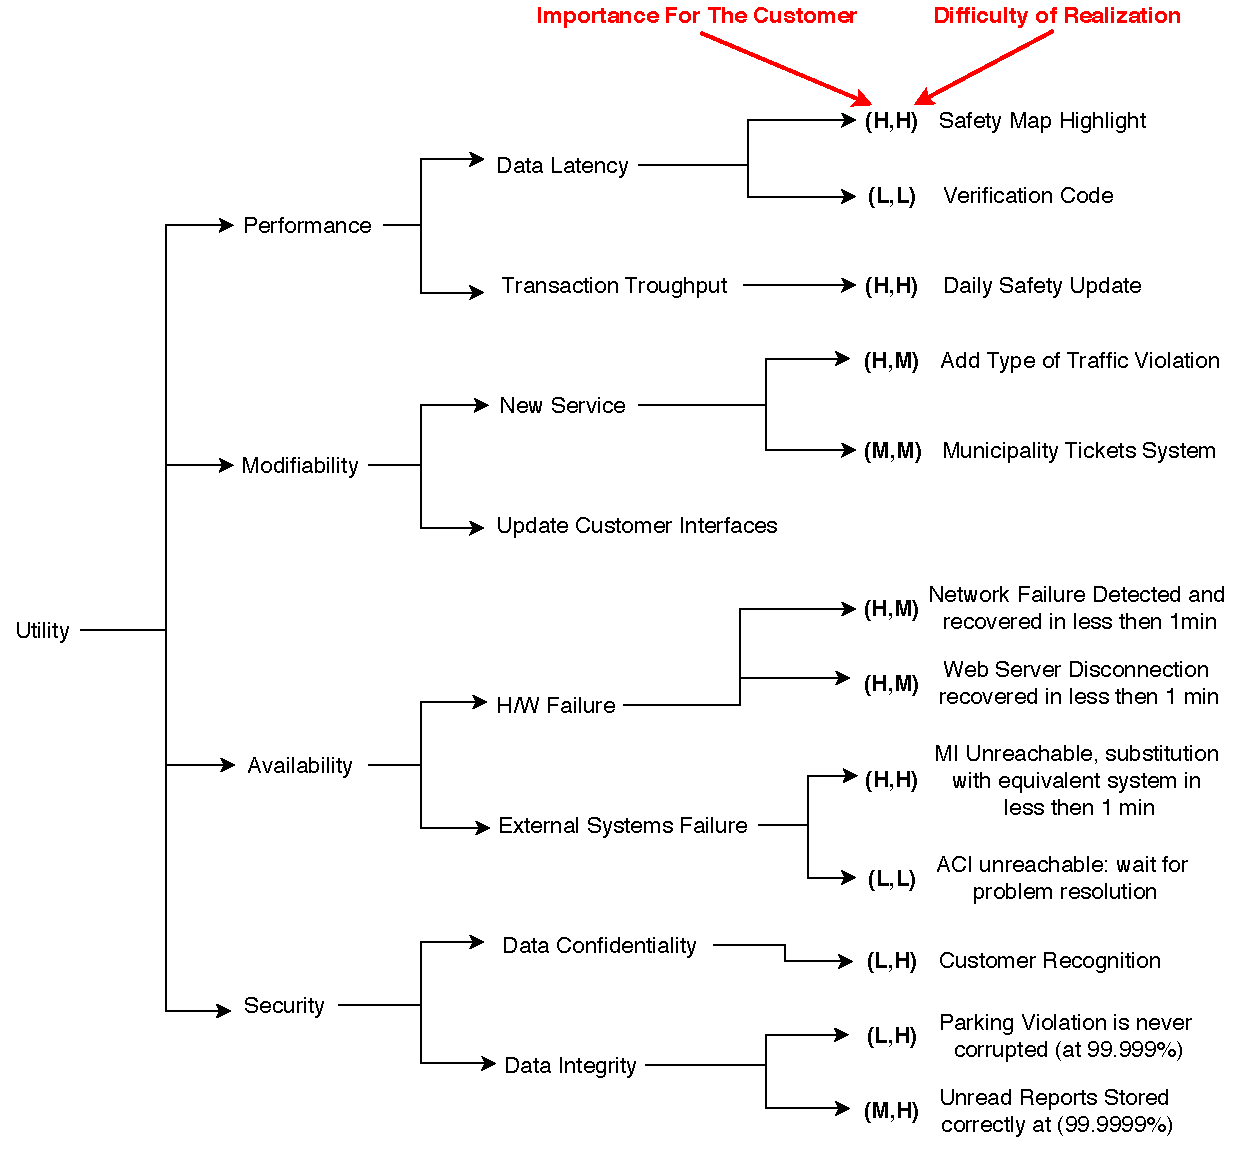
\includegraphics[scale=0.57]{utilityTree}
			\caption{\label{fig:utilityTree} Utility Tree}
		\end{figure}
		
	\subsubsection[Plan Definition]{\hyperlink{toc}{Plan Definition}}
		\label{sec:planDefinition}
		
		\begin{figure}[h!]
			\centering
			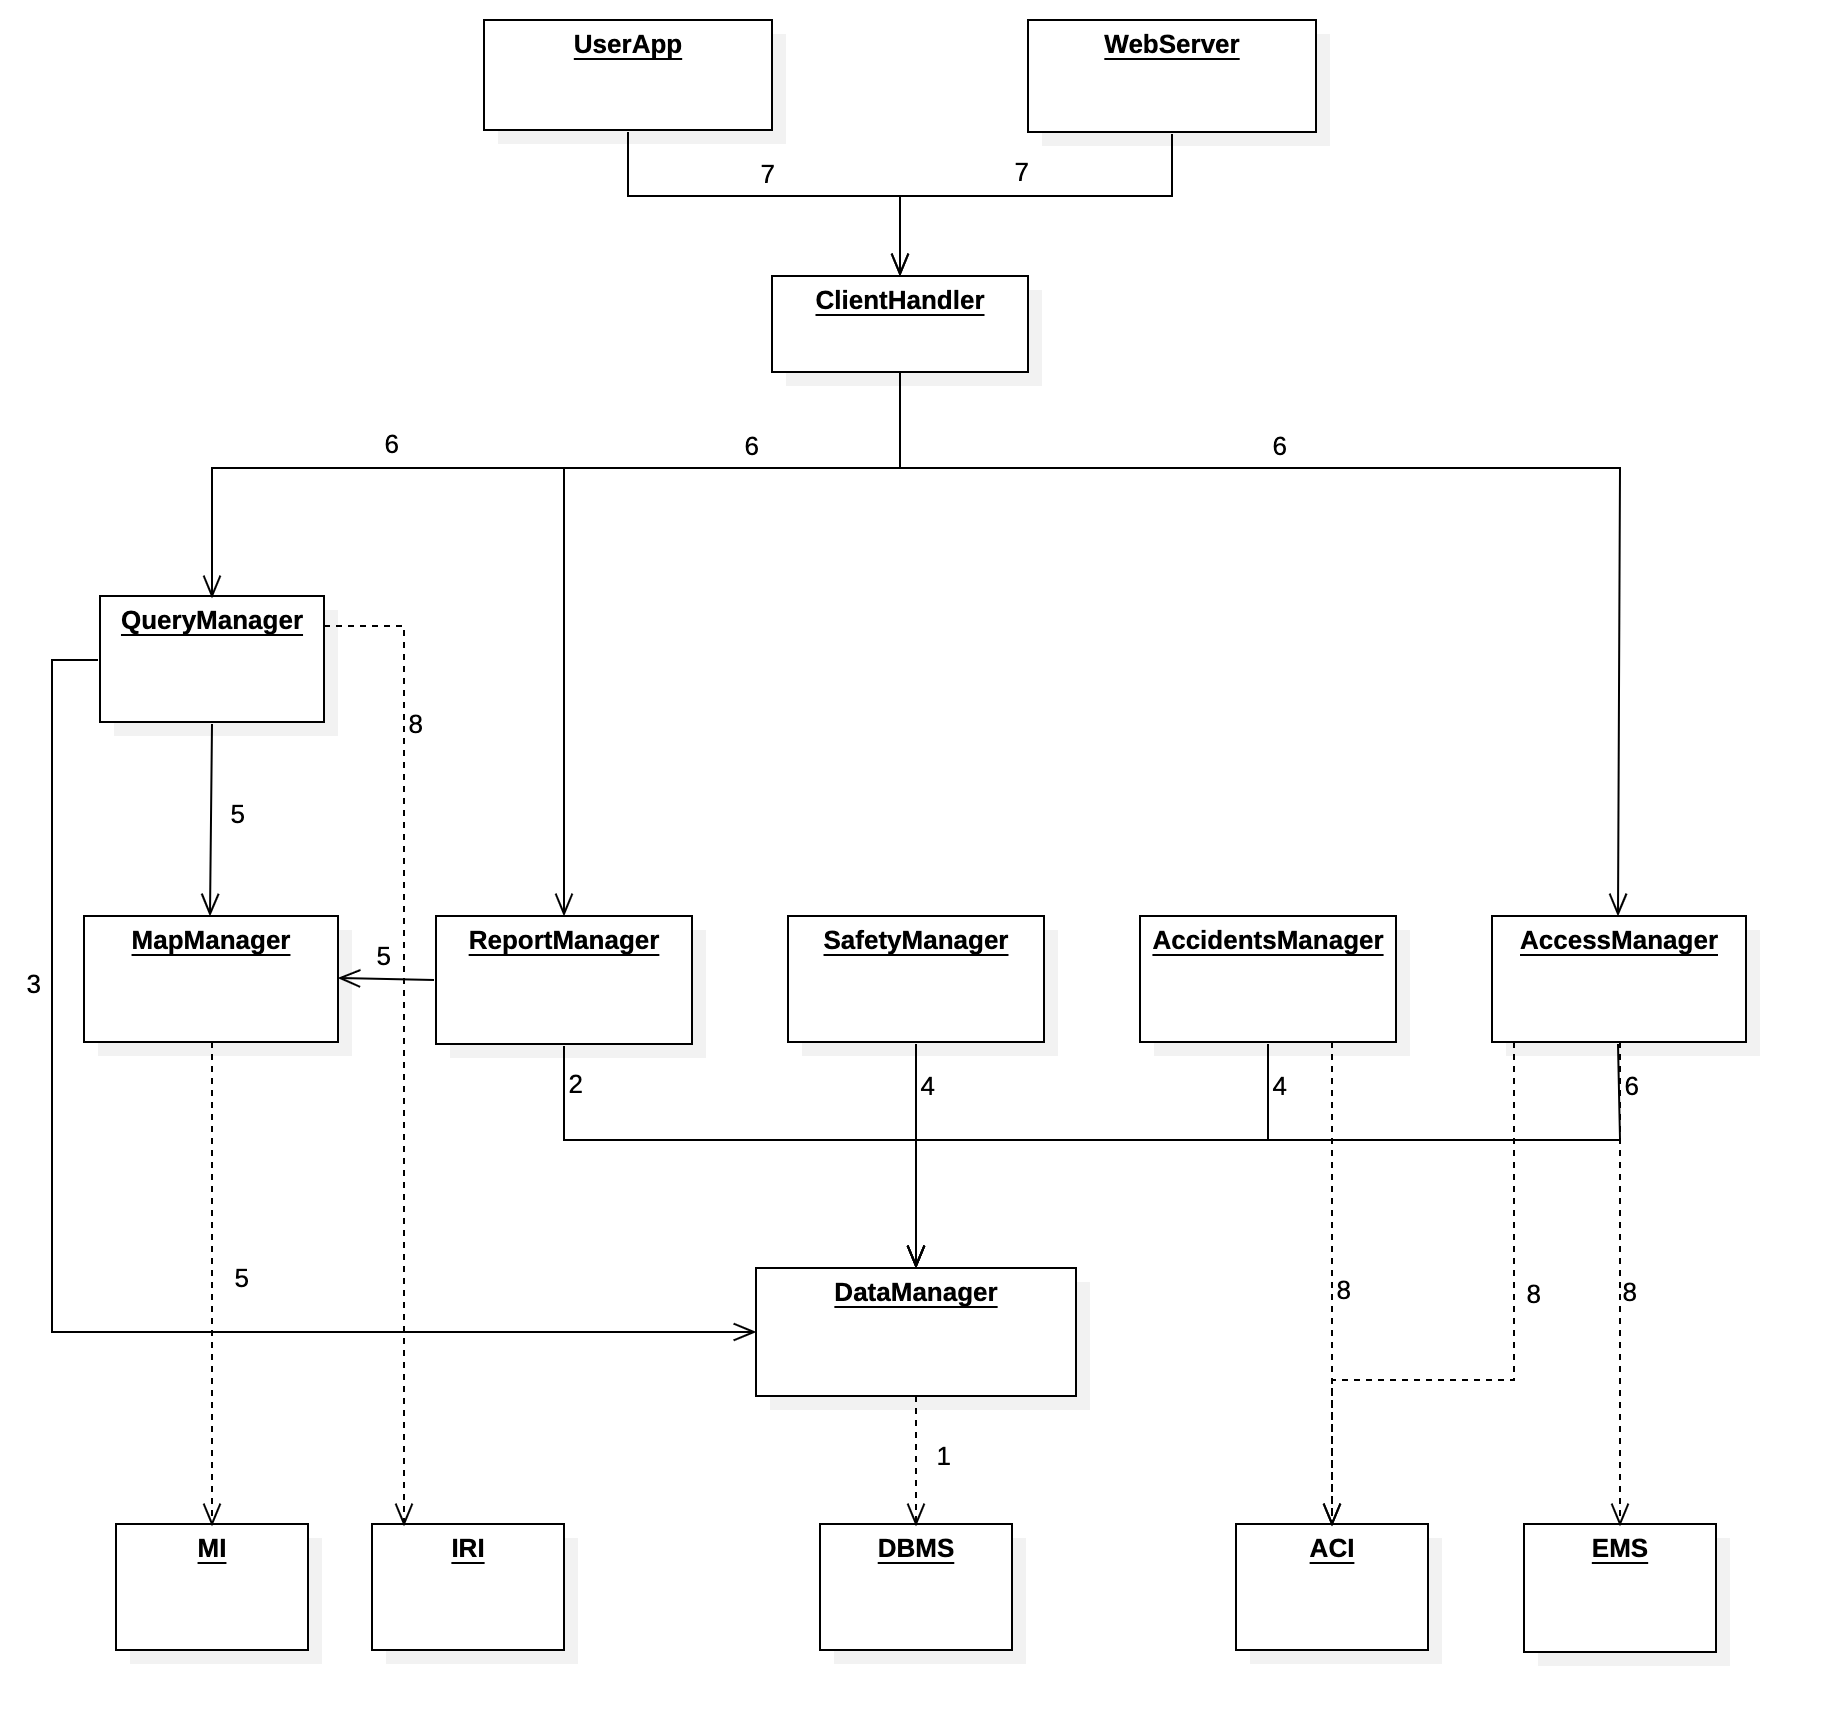
\includegraphics[scale=0.17]{/diagrams/useRelationHierarchy.png}
			\caption{\label{fig:useRelationHierarchy} Use Relation Hierarchy Diagram}
		\end{figure}
	
		\begin{enumerate}
			\item The first component we plan to implement is DataManager. This choice is due to the fact that this particular component is responsible of all the interactions with the database and it is needed by the majority of all the other components in the ApplicationServer, being the very leaf of the tree, as shown in the diagram. Then it will be integrated with the DBMS and thus tested.
			
			\item Then, the ReportManager component will be implemented because its role is quite crucial for the whole system. It provides in fact the core functionality, allowing users to notify authorities of violations. Its integration with the DataManager will follow as soon as possible. It is important to highlight the fact that ReportManager needs MapManager only to retrieve the name of the street from the position of a reported violation. Because of this, it is quite simple to generate a stub for MapManager and test ReportManager anyway. The components designed to handle the interactions with external interfaces are planned to be implemented later on, mainly because they’re not that “intelligent” and external APIs are well documented. 
			
			\item Next step is implementing QueryManager, another extremely important component, and probably the most complex one. It needs to be fully implemented and tested as soon as possible, and integrated with DataManager because of course queries rely a lot on the DBMS. With regard to MapManager, the same thing as point 2 applies here: the difference is that now MapManager is needed for path finding and map retrieval and thus is a little bit more crucial. This is the reason why the integration of MapManager with the interacting components will have to be done in the very following steps.
			
			\item In order to complete the development of the most important functionalities, we now plan to implement and test AccidentsManager and SafetyManager, and integrate them with DataManager. They are actually not too complex components, so this operation should be quite fast. The idea is to integrate AccidentsManager and ACI later on.
			
			\item It is now time to complete the implementation of MapManager and integrate it with the two components that use it (ReportManager and QueryManager) and with the external MapInterface. Excluding the interactions with the remaining external interfaces and the registration/login services, the system is now ready to provide all the functionalities.
			
			\item Now that the internal logic is complete, we plan to realize the components that interact with clients. Therefore, ClientHandler and AccessManager will be implemented, tested and integrated together and with all the components they interact, that are ReportManager, QueryManager and DataManager. Thanks to the section related to the user interfaces (\ref{sec:userInterfaceDesign}) we give the developers an illustration of how the interaction with the clients have to occur in order to provide the functionalities of the system. As already said in that section, the graphical interface can be modified and beautified with the skills of the developers as long as they stick on the way in which the functionalities have to be provided.
			
			\item Since ClientHandler is now fully tested, we could integrate it with the UserApp and the WebServer.
			
			\item As the last step, we plan to integrate all the remaining external interfaces with the internal components that use them: QueryManager will be integrated with IRI, AccessManager and AccidentsManager will be integrated with the AuthorityCommonInterface, and finally AccessManager with EMS. 
		\end{enumerate}